\documentclass[10pt,twocolumn,letterpaper]{article}

%\usepackage{cvpr}
\usepackage{times}
\usepackage{epsfig}
\usepackage{graphicx}
\usepackage{amsmath}
\usepackage{amssymb}
\input defs.tex
% Include other packages here, before hyperref.

% If you comment hyperref and then uncomment it, you should delete
% egpaper.aux before re-running latex.  (Or just hit 'q' on the first latex
% run, let it finish, and you should be clear).
\usepackage[pagebackref=true,breaklinks=true,letterpaper=true,colorlinks,bookmarks=false]{hyperref}

\bibliographystyle{alpha}


% \cvprfinalcopy % *** Uncomment this line for the final submission

%\def\cvprPaperID{****} % *** Enter the CVPR Paper ID here
%\def\httilde{\mbox{\tt\raisebox{-.5ex}{\symbol{126}}}}

% Pages are numbered in submission mode, and unnumbered in camera-ready
% \ifcvprfinal\pagestyle{empty}\fi
\begin{document}

%%%%%%%%% TITLE
\title{Convex Optimization for Computer Vision Data Selection}

\author{David Jose Florez Rodriguez\\
Stanford University\\
Stanford, CA \\
{\tt\small sirdavid@stanford.edu}
% For a paper whose authors are all at the same institution,
% omit the following lines up until the closing ``}''.
% Additional authors and addresses can be added with ``\and'',
% just like the second author.
% To save space, use either the email address or home page, not both
\and
Gabriel Magaña\\
Stanford University\\
Stanford, CA\\
{\tt\small gdmagana@stanford.edu}
\and
Benjamin Martinez\\
Stanford University\\
Stanford, CA\\
{\tt\small benjm@stanford.edu}
}

\maketitle
%\thispagestyle{empty}

%%%%%%%%% ABSTRACT
\begin{abstract}
We explore a novel, convex, data selection optimizer's potential to provide tailored datasets in medical imaging applications. We compare our novel method to the previously successful Truncated Monte Carlo Data Shapley method (TMC), a control of randomly sampled data and a larger raw dataset. The predictors include various convolutional models trained from scratch and some previously successful image classifiers fit to our specific problem via transfer learning. Our method outperformed TMC across multiple metrics including accuracy, loss, and efficiency.
\end{abstract}

%%%%%%%%% BODY TEXT
\section{Introduction}

 X-ray classification is fundamental in scheduled and emergency procedures throughout the world. Due to the life-or-death importance of this practice, anything below the best accuracy and the fastest response times will have great costs for society; unfortunately, radiologists are in low supply and machine learning models looking to step in are finding the silos of medical data sets limiting. Due to unique imaging configurations and demographic variations across different hospitals' patient population, it is difficult (even with IBM / GE level funding)\footnote{IBM Watson and GE Edison are two of the biggest competitors in the AI in healthcare space, but none have covered a large fraction of the image classification market} to create models with steady performance in clinics across the globe.
 
  We present the `Convex Pseudo-Spread Maximizer' (CPSM) method. Employing the cvxpy python library\footnote{a modelling language robustly defining and solving convex optimization problems leveraging the work of \cite{cvxrewrite}} we define the `pseudo-spread' as a metric for the spread and distribution density of a dataset in a defined feature space and maximize said spread such that no more than a fixed number of the training samples may be used.
  
  All code is available at \cite{dfgit}.
  
 \section{Related Work}
 
 \subsection{Data Selection}
 
 In the present healthcare supply and demand mismatch scenario, data selection could prove essential. 
 A survey of available methods in \cite{datasel} explores the problem of picking valuable data points from a dataset to optimize final predictor performance. Two pre-training statistical methods for evaluating samples' potential contribution to a tailored dataset are compared to the staple `Leave-one-out' algorithm, which iteratively trains models on subsets of the whole database and evaluates the contribution of those data points not in the subset via the difference in performance when training on the subset and when training on the whole dataset. 
 
 
 The Truncated Monte Carlo Data Shapley (TMC) method presented in \cite{datashapley} fulfills equity metrics defined in its paper and succeeds in appointing data values that accurately portray outliers and noisy samples. If a successful AI could classify X-rays into diagnoses without a massive training set, the growth of AI assisted radiology stands a better chance of keeping up with radiology demand. Working toward this goal, data selection algorithms seek the most informative data so the dataset size threshold for accuracy decreases. 
 
 TMC's performance in enhancing multi-class image classifiers is promising for the research at hand. TMC's data selection is the standard against which we'll compare our CPSM algorithm.
 

\subsection{Transfer Learning}

On top of the limited data issue, medical imaging scans also vary widely across regions. Training many models that specialize in different hospitals' patients may be easier than training a massive model. For this reason, and to leverage powerful, fully-trained models from outside of healthcare, transfer learning is important. The survey of existing methods in \cite{surveytransfer} showcases the most successful practices in this subfield of computer vision. This work's transfer learning implementations employ their general guidelines to transfer learning across image categories: the farther away the images in the desired training at hand are from the original training set of the model to be transferred, the more layers one needs to retrain in the transferred model. 

This work follows a specific retraining scheme from \cite{surveytransfer} where the desired training data is of a completely separate category and different dimensions than the original training data of the model: we sandwich a ResNet from \cite{resnet} and an EfficientNet from \cite{efficientnet} between convolutional and fully-connected layers.

\subsection{AI on X-rays}

The original architectures for shallow training were based on smaller versions of successful models presented in \cite{aixray} and \cite{aidiag}. Particularly, hyperparameter testing of convolutional filter size and the relative count of convolutional to neural layers in our raw convolutional networks were inspired by these works.

\section{Methods}

\subsection{Data}
This work uses the PADCHEST\cite{padchest} dataset and chose 7 common diagnosis labels to train our model to detect. 
These labels are: Normal, COPD signs, pneumonia, scoliosis, infiltrates, cardiomegaly, and pleural effusion. 
Our eighth label we trained on was 'OTHER', or if the patient had a diagnosis not among our other 7. The amounts for each label are referenced in Figure~\ref{fig:bar}.
We resized each image to be 1800 by 1800 since the dataset had lots of variation in size, since this is what was recommended by doctors we surveyed on what resolutions were sufficient for diagnoses. For example, Figure~\ref{fig:paimg1} is a chest xray image.
Out of the 1000 images, we used 600 as a training set and 200 as a validation set for our architecture and hyperparameter search. 
\begin{figure}[!htb]
    \centering

    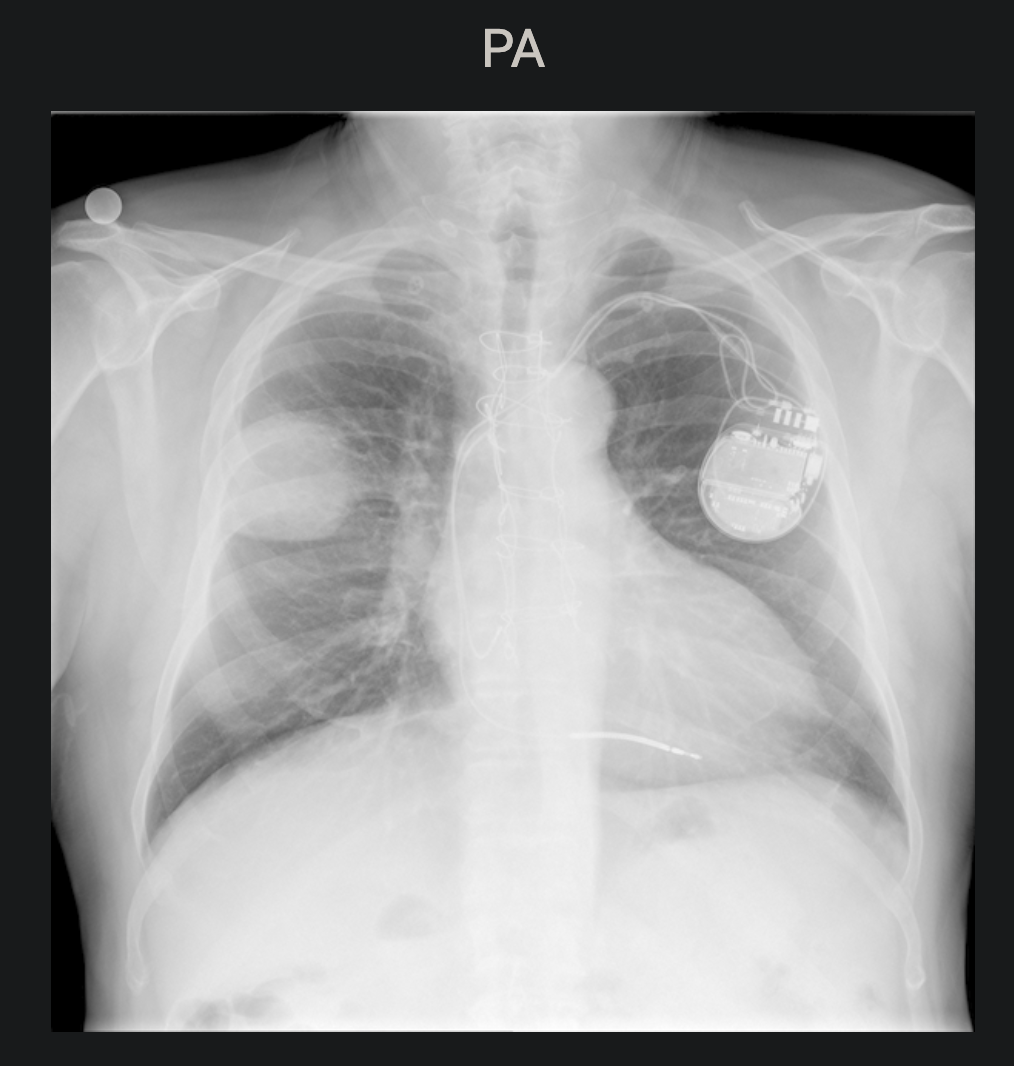
\includegraphics[width=6cm]{latex/figs/paimg2.png}
    \caption{A sample chest image from the dataset, this one with labels [‘pneumothorax’, ‘pulmonary mass’], which in our data is represented as only OTHER}
    \label{fig:paimg1}
\end{figure}
\begin{figure}[!htb]
    \centering

    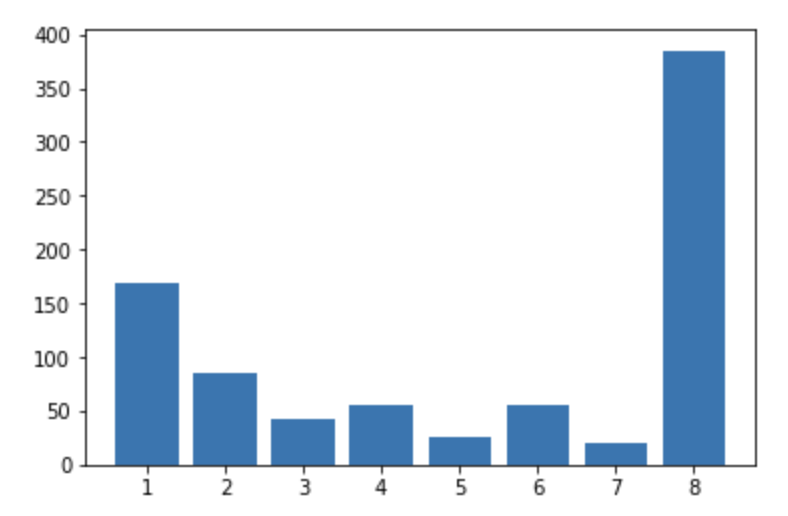
\includegraphics[width=6cm]{latex/figs/bar.png}
    \caption{The amount of each diagnosis label in our training set, with labels 1-8 being the aforementioned labels in that order}
    \label{fig:bar}
\end{figure}


\subsection{Model and Hyperparameter Shallow Search}
Initially, various model architectures with randomly generated hyperparameters train for $4$ epochs (denoted `shallow' training). Figure ~\ref{fig:CNN}, ~\ref{fig:transfer} shows the architectures explored. For regularization and learning rate, each model instance generated two random values from a uniform distribution $r_l, r_r \in \left[ 2,7\right]$ . Regularization and learning rate were set to $10^{-r_l}$ and $10^{-r_r}$ respectively. A few of the models and hyperparameters' in shallow training can be found in figures ~\ref{fig:model1},~\ref{fig:model2},~\ref{fig:model3} in the appendix.
\begin{figure}[!htb]
    \centering

    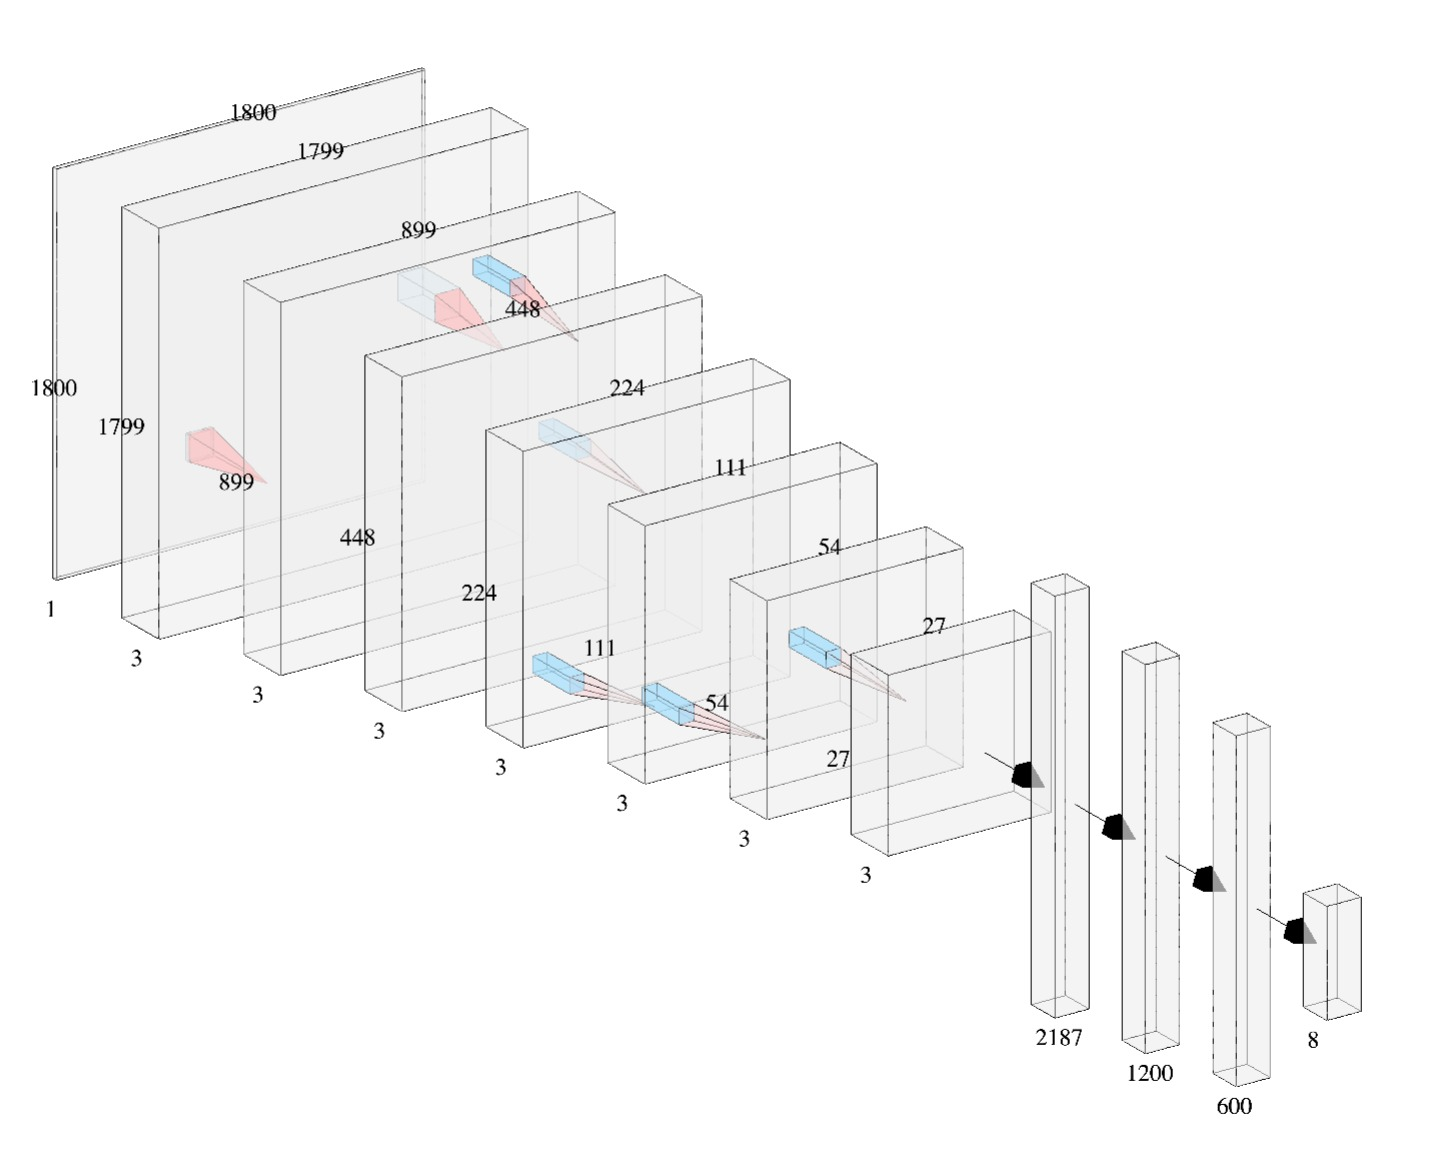
\includegraphics[width=6cm]{latex/figs/CNN_architecture.jpeg}
    \caption{Novel CNN architecture experimented with varied filter sizes and dense layer sizes.}
    \label{fig:CNN}
\end{figure}

\begin{figure}
    \centering

    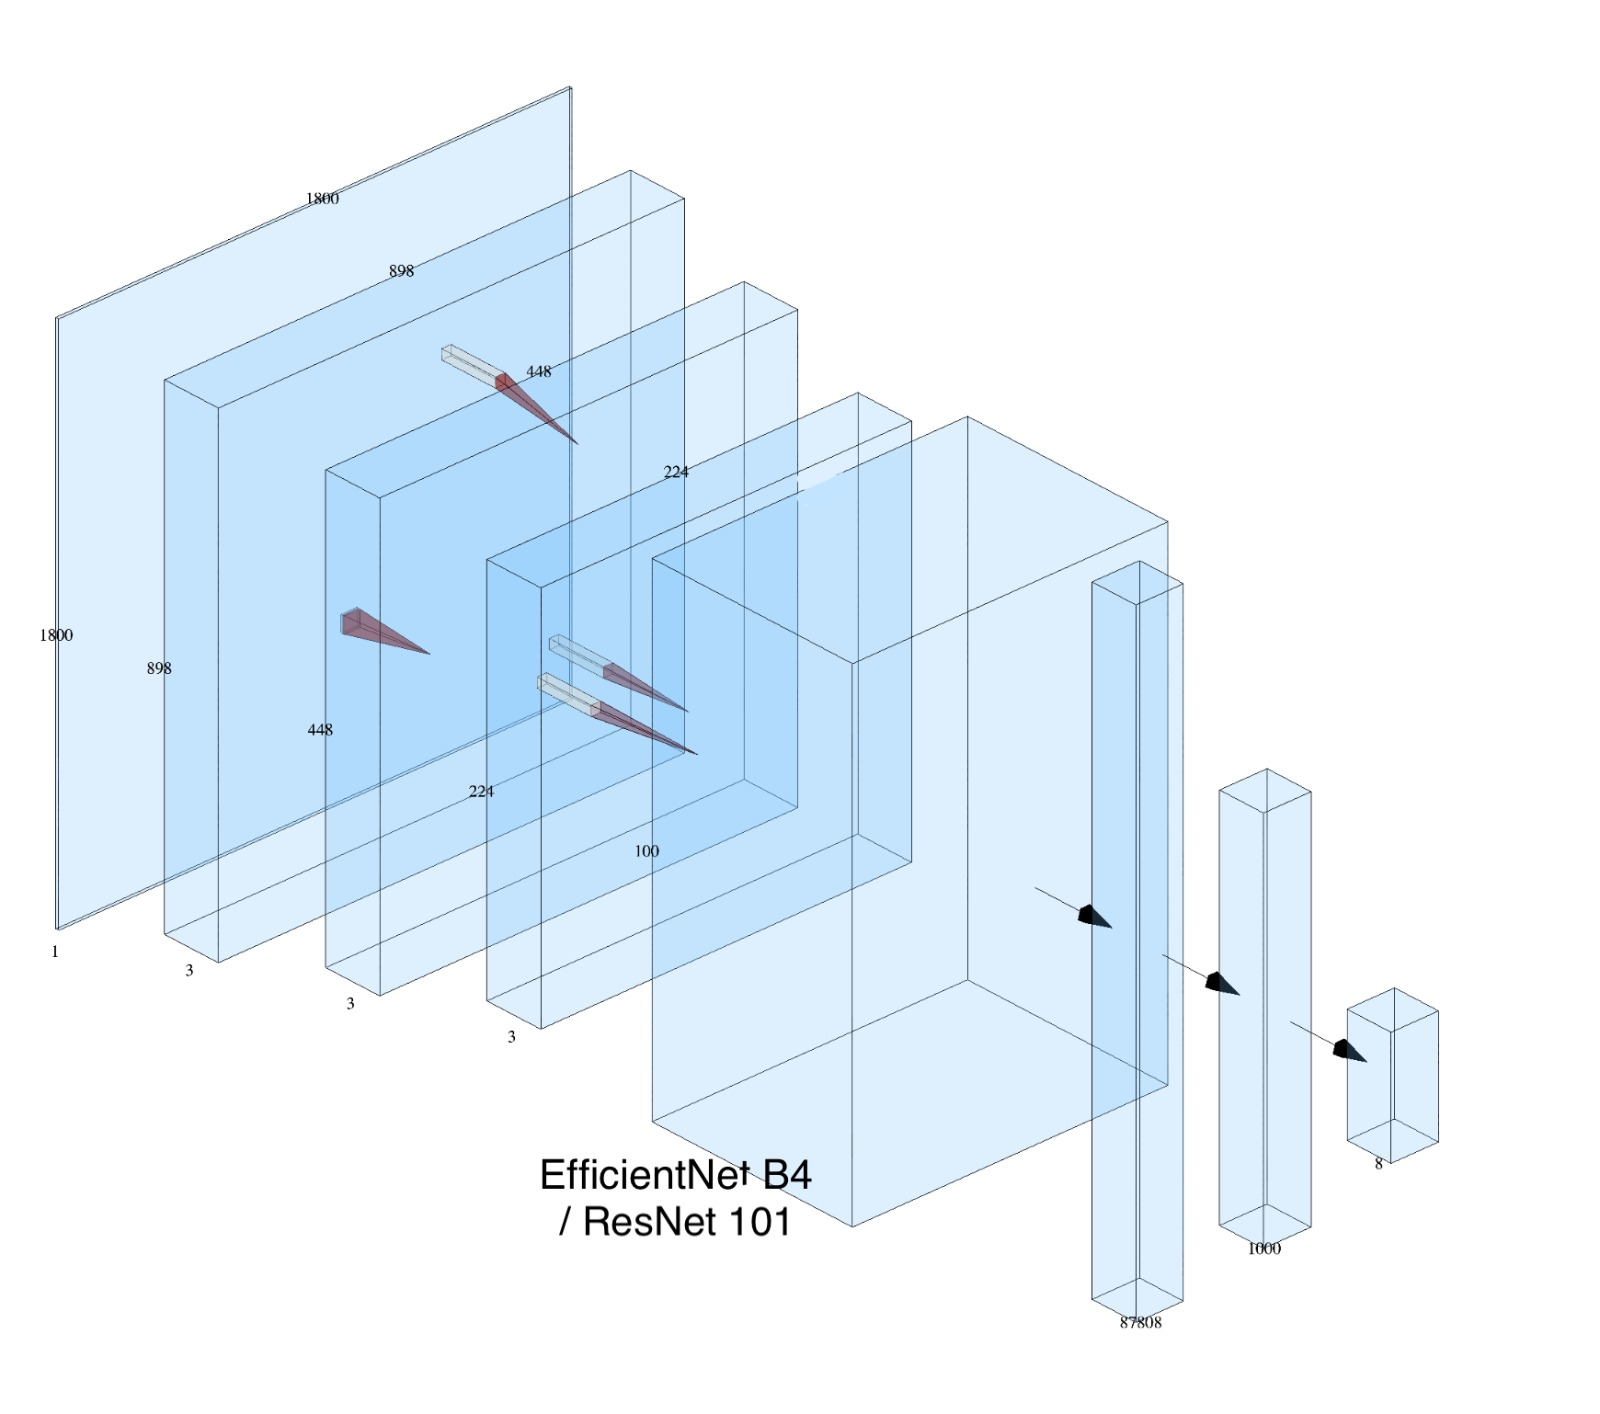
\includegraphics[width=6cm]{latex/figs/transfer_architecture.jpeg}
    \caption{Transfer learning architecture using a CNN as input to either EfficientNetB4 or ResNet101 with custom dense layers.}
    \label{fig:transfer}
\end{figure}

Best model and hyperparameters were determined by training accuracy after the set epochs and the general slope of the training curve. Models with high training accuracy and no sign of plateauing performance moved on to deeper training. Performance of various models and hyperparameter configurations are shared starting with figure ~\ref{fig:model1} in the Appendix.




\subsubsection{Transfer Learning and Deeper Training}

The models that succeeded in few training epochs inspired the architectures and hyperparameters for the transfer learning models. With both ResNet and EfficientNet, a set of convolutional layers resize our input data (X-rays are much higher resolution than the ImageNet data these models trained on). These convolutional layers also aim to capture meaningful image features to feed into the imported models. At the output end of the imported models, their first dense layer feeds into custom dense layers, which result in an output of the appropriate size for this work.

In the next stage of training, convolutional models built from scratch (hereby denoted `raw' models) trained for $15$ epochs with the goal of exhibiting the learning capacity to overtrain on the model. In practice, transfer models only trained for $7$ epochs, as previous experiments learned that these models rapidly plateau.

The best performing raw and transfer model after this stage of training became the predictors that evaluated our data selection methods. We use subsets of $75$ and $150$


\subsection{Convex Pseudo-Spread Maximizer}

The novel data selection method in this work acts on a set of $M$ vectors of size $K$ stored in a  matrix $A\in \reals^{M \times K}$. We obtain such vectors by extracting the first dense layer from our best model after the overfitting stage of training. The hope is that each image's representation in this feature space is meaningful for our application and can convey which images are highly similar and which are outliers in the dataset. The t-SNE method\cite{tsne} provides a $2$D representation of our data in this feature space in figure ~\ref{fig:tSNE}.
\begin{figure}
    \centering

    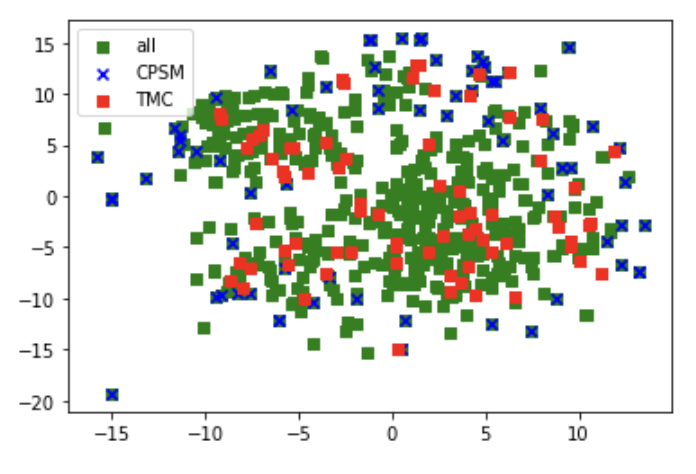
\includegraphics[width=6cm]{latex/figs/tSNE.png}
    \caption{t-SNE depiction of image feature space}
    \label{fig:tSNE}
\end{figure}

The problem of data selection aims to choose $N$ data points out of a larger dataset with $M>N$ samples such that the learning a predictor can obtain from training on these $N$ points is maximized. A metric on which to evaluate data points is necessary for such an algorithm, however.

We define the pseudo-spread $$S = \sum \omega^T D + \frac{\alpha}{N} \sum \omega^T \left((A-\Theta)^T(A-\Theta)\right),$$

whose variables we define below.

The matrix $\omega \in \{0,1\}^{M \times M}$ is the variable in our convex optimization, its diagonal stores the selection of data points encoded in binary. The mechanism here is as follows: if $\omega_{i,i}==1$, sample $i$ is in CPSM's selected subset of $A$, and if $\omega_{i,i}==0$, sample $i$ is excluded.

The matrix $D \in \reals^{M \times M}$ is a distance matrix which keeps track of how far each data point is from each other in the feature space. One iterative method of obtaining $D$ is computing $$D_{i,j} = (A_{i}-A_{j})^T(A_{i}-A_{j})$$ for all values of $i$ and $j$. 

The scalar $\alpha$ is an empirically derived hyperparameter to be discussed below. 

The matrix $\Theta \in \reals^{M \times K}$ is a tiled version of the vector $\theta \in \reals^{K}$ which is the median of $A$; therefore $$\Theta = \begin{bmatrix} \theta^T \\ \vdots \\ \theta^T.
\end{bmatrix}$$

Finally, we pose the problem of finding the best $N$ samples from $A$ as follows in cvxpy:
\begin{quote}
 
    \[
        \begin{array}{ll}
            \mbox{Maximize} & S,
        \end{array}
    \]
    such that $0 \leq \omega \leq I_M$, and $\sum \omega <= N$ 
\end{quote}
where $I_M$ is the identity matrix with $M$ columns and the relevant inequalities denote element-wise relations.

%   Ndata,Ddata = x1.shape
%   diag = cp.Variable((Ndata,Ndata))
  
%   med = np.median( x1, 0, keepdims=True)
%   print(med.shape)
%   MEDIAN = np.tile(med,(Ndata,1))

%   D =   2*np.sum(x1**2,1,keepdims=True) - 2* x1 @x1.T
%   constraint = [cp.sum(diag)<=N, diag<=np.eye(Ndata), diag >=0]
%   obj = cp.Maximize(cp.sum(diag @ D) + alpha/N*cp.sum(diag @ cp.square( x1 - MEDIAN)) )
\subsubsection{CPSM Motivation}
The pseudo-spread can be dissected into a weighted sum of two metrics: $S_1$, a masked sum of all the vector-to-vector distances $\sum \omega^T D$, and $S_2$, a masked, modified variance computation $\frac{1}{N} \sum \omega^T \left((A-\Theta)^T(A-\Theta)\right)$. 

The binary mask (which we later constrain non-zero values only in the diagonal) $\omega$ serves to vary $S$ according to which samples are present in CPSM's chosen subset of $A$. The masked sum of distances then ensures that two samples with very similar features are not both included. For low values of $N$, this metric would choose only points of the perimeter of a distribution, for example. And the masked, modified variance simply aims to capture the variance of the selected points. The median $theta$ drives this metric, rather than the mean, because a live computation of the mean inside the optimization metric could make the object of the optimization non-convex. Having to keep a fixed metric in the variance computation, it's better to select the median. The mean could change significantly if certain outlier are excluded from CPSM's selected subset, but the median should be more robust.

The hyperparameter $\alpha$ could be tuned via iterative experiments, but is set based on the relative sizes of the $S_1$ and $S_2$ components of $S$. A loop computed the ratio of $S_1$ to $S_2$ for one hundred randomly generated matrices with the same mean and standard distribution as dataset $A$. On average, $S_1$ was about $3000$  bigger than $S_2$, so $\alpha = 3000$ in our experiments.

\subsection{Truncated Monte Carlo Data Shapley}

We employ the TMC method using the best performing model from the deeper training stage. For a robust benchmark of data selection, the algorithm trained hundreds of instances of the same model trained on different training sets, totaling over 40 hours of computing time and thousands of training-validation sequences. The details of the algorithm are best explained in \cite{datashapley}, but in short it is an iterative algorithm that first validates without training, adds a random sample to the training set, and validates again. This is repeated until performance plateaus, and each improvement in performance becomes an approximation of the Data Shapley data value of the sample that was added. Repeating this algorithm hundreds of times provides a list of approximations for each sample's Data Shapley value. Each sample's average Data Shapley value is the algorithm's approximation for the sample's valued in data selection.



\section{Results}



The raw models trained with CPSM-derived data perform the best out of all models. Of the data selection algorithms on 75 samples, CPSM on a CNN performed with 10\% better accuracy than the next best algorithm, TMC on a CNN, with their performances being ~51\% and ~44\% respectively. CPSM and TMC on CNN are both significantly higher than their correspondents on transfer learning with ~15\% and ~20\% higher accuracy respectively. Similar patterns can be seen on training with 150 samples.

The CPSM and TMC data selection schemes yielded similar results in most cases, but one must note that the CPSM method provides results in under $5$ minutes, whereas the TMC method requires dozens of hours of computing time. Most transfer learning models underperformed the raw models and had no learning after the first epoch. This was probably a result of poor transfer learning practices. Supporting the value of data selection, all raw models trained on either TMC or CPSM outperform their counterparts trained on random data. CPSM using transfer learning outperformed their random data counterpart by a factor of ~2, CPSM using CNNs outperformed their random data counterpart by a factor of ~1.45. And TMC using transfer learning outperformed their random data counterpart by a factor of ~1.3, TMC using CNNs outperformed their counterpart by a factor of ~1.2.

\begin{figure}[!htb]
    \centering

    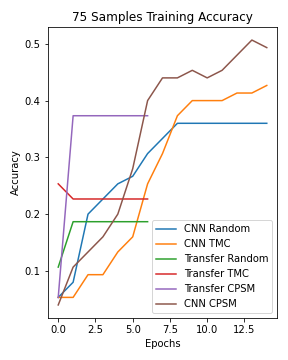
\includegraphics[width=6cm]{latex/figs/75_Accuracies(1).png}
    \caption{Models' accuracy on 75 samples.}
    \label{fig:data_selection_75}
\end{figure}

\begin{figure}[!htb]
    \centering

    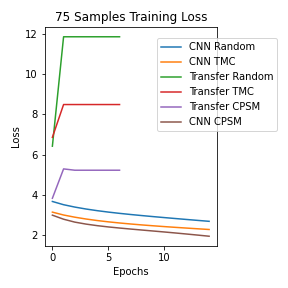
\includegraphics[width=6cm]{latex/figs/75_Losses(1).png}
    \caption{Models' losses on 75 samples.}
    \label{fig:data_selection_75}
\end{figure}

\begin{figure}[!htb]
    \centering

    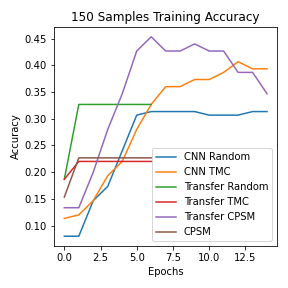
\includegraphics[width=6cm]{latex/figs/150_Accuracies(1).png}
    \caption{Models' accuracy on 150 samples.}
    \label{fig:data_selection_150}
\end{figure}

\begin{figure}[!htb]
    \centering

    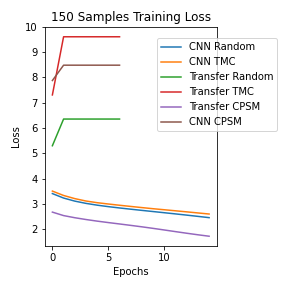
\includegraphics[width=6cm]{latex/figs/150_Losses(1).png}
    \caption{Models' losses on 150 samples.}
    \label{fig:data_selection_150}
\end{figure}

\section{Conclusion}

Our novel CPSM data selection method outperformed the benchmark TMC method. CPSM runs over $100$ times faster, due to its closed form convex optimization nature, but does require ample system memory. This same closed form nature also guarantees the global optimal value of its data selection for maximizing the pseudo-spread heuristic. As CPSM's data selection was based on a feature space resulting from training, the results suggest that this feature space, over-trained on a few dozen epochs, are able to learn meaningful features in the space.

Future work will look at better transfer learning to properly compare raw models with existing models, and a comparison to models trained on datasets orders of magnitudes larger than our own. Additionally, the CPSM and TMC methods could both run on segmented data for each class in the classifier. Experiments with such an implementation may provide better data selection.

\section{Acknowledgements}
This work would not have been possible without the medical expertise of Dr. Manuel Acosta and Dr. Antonio Bueso. Additionally, the EE364A course by Stephen Boyd inspired our CPSM method possible.

{\small
\bibliographystyle{ieee}
\bibliography{egbib}
}
\newpage
\section{Appendix}



\begin{figure}[!htb]

    \centering
    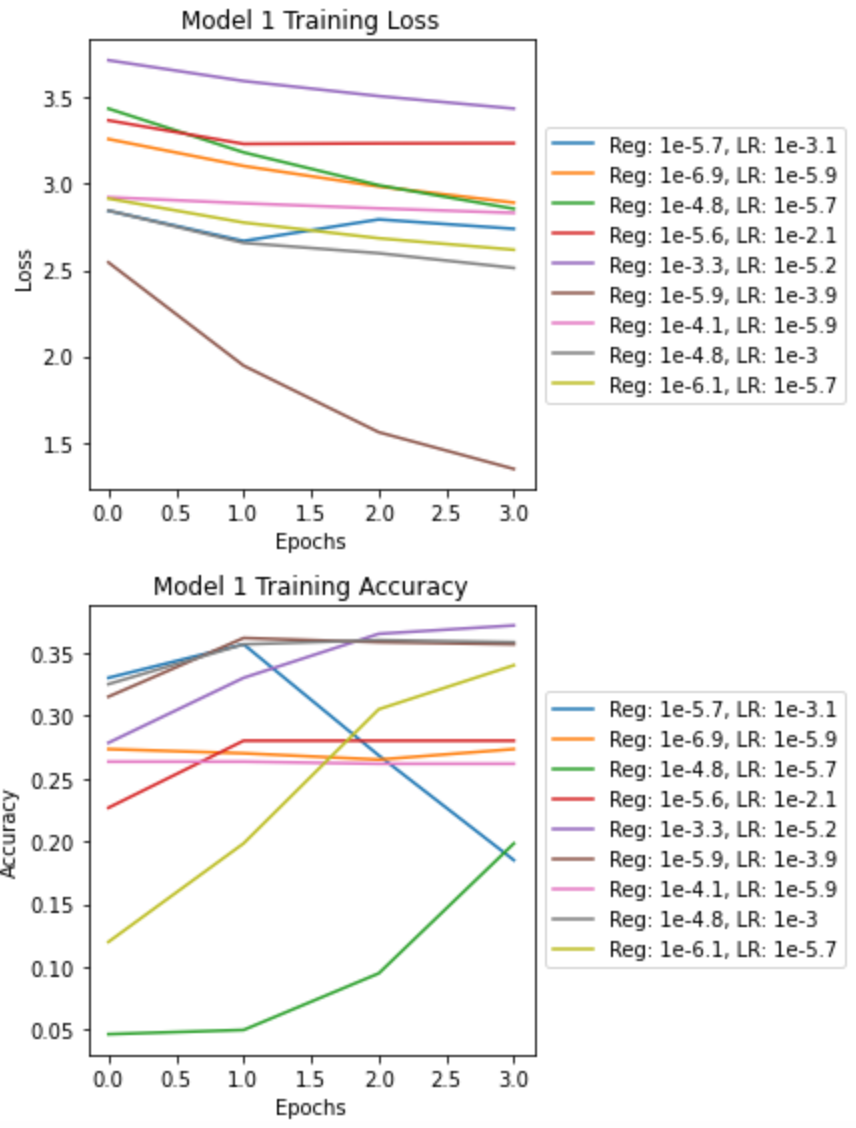
\includegraphics[width=6cm]{latex/figs/model1.png}
    \caption{Models' loss and accuracy over epoch. Model 1 has filter size 2, a dense layer 1 of size 1000, and a dense layer 2 of size 800. }
    \label{fig:model1}
\end{figure}
\begin{figure}[!htb]

    \centering
    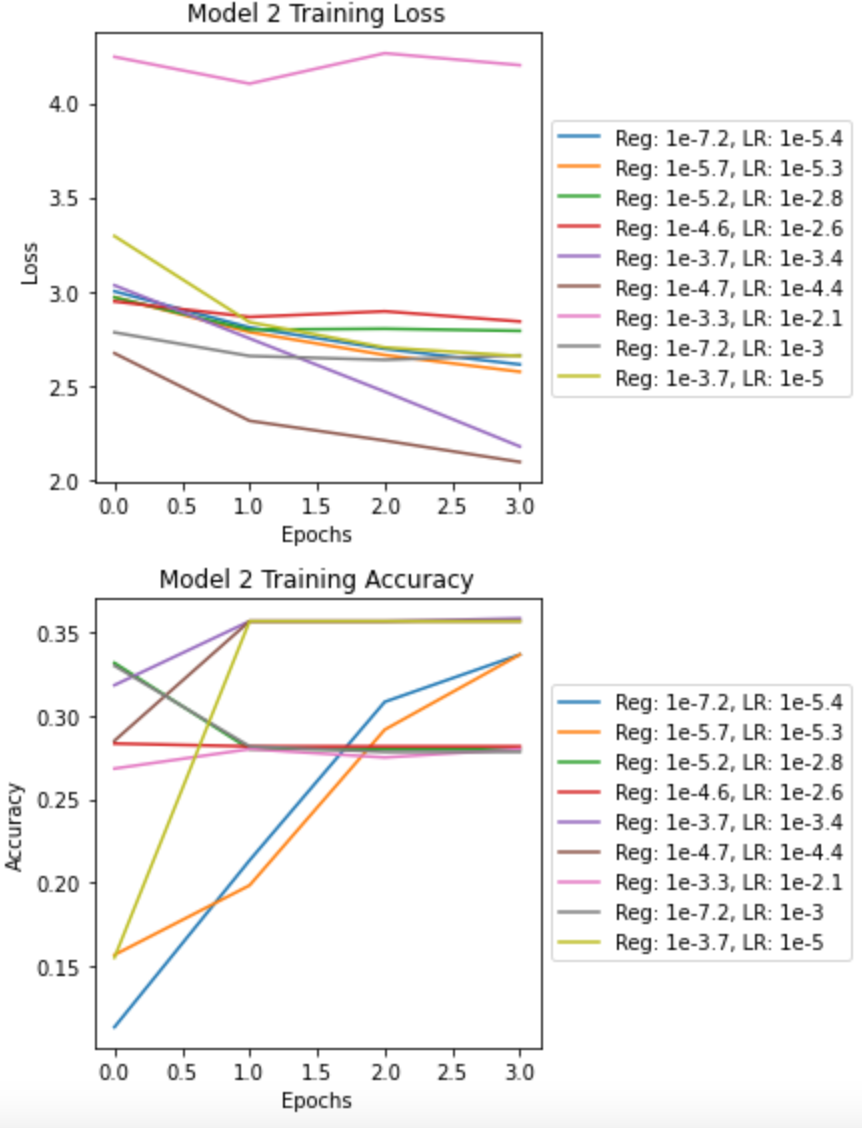
\includegraphics[width=6cm]{latex/figs/model2.png}
    \caption{Models' loss and accuracy over epoch. Model 2 has filter size 3, a dense layer 1 of size 1000, and a dense layer 2 of size 800. }
    \label{fig:model2}
\end{figure}
\begin{figure}
    \centering

    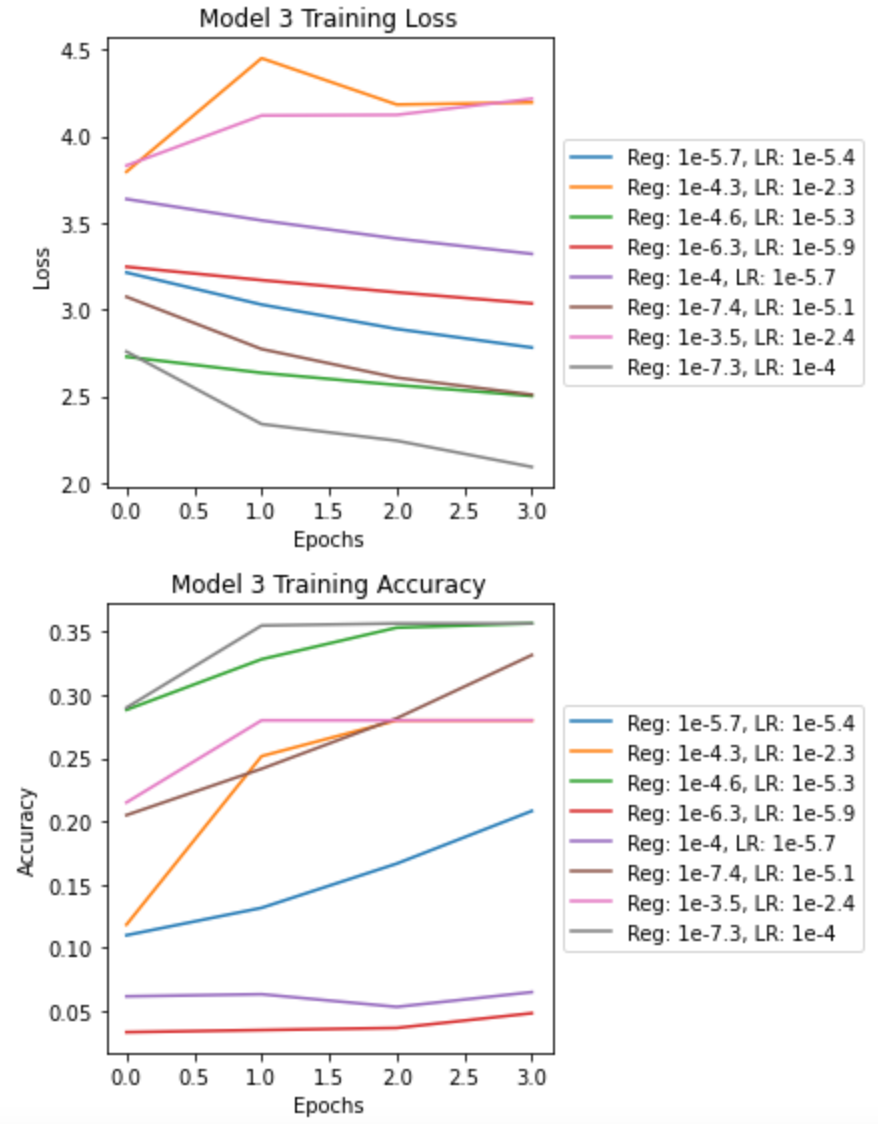
\includegraphics[width=6cm]{latex/figs/model3.png}
    \caption{Models' loss and accuracy over epoch. Model 3 has filter size 2, a dense layer 1 of size 1200, and a dense layer 2 of size 600.}
    \label{fig:model3}
\end{figure}





\end{document}